\documentclass{article}
\usepackage{tikz, comment}
\usepackage{pifont}
\usepackage{fontspec}
\usetikzlibrary{arrows, decorations.markings, decorations.pathreplacing}
\begin{comment}
:Title: Not defined yet
:Tags: area using polar coordinates, polar integral formula ;sohcahtoa;polar form of a complex number;cosine, cos ;sine, sin 
:Prob: 0.4679;0.4058;0.3958;0.3957;0.3756
:Author: Prof.Hu Ji-shan, HKUST
:Slug: No name yet

Description Here.........
\end{comment}
\begin{document}\centering

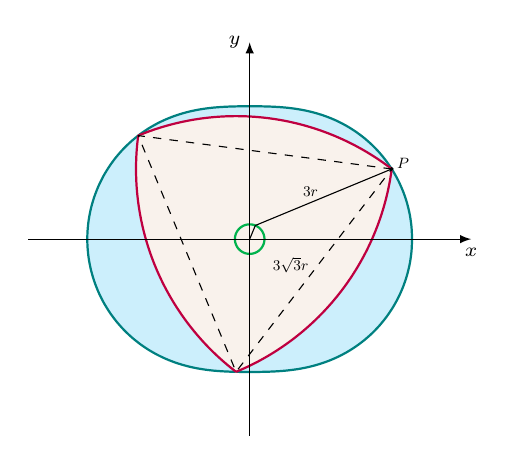
\begin{tikzpicture}[>=latex,xscale=.5*1.25, yscale=.5*1.25][font=\sf\small]

%\draw[xstep=1cm,ystep=1cm,color=gray!80] (0, -1) grid (8, 8);

\draw[thick, teal, fill=cyan!20, samples=100, smooth, domain=0:2*pi, variable=\t]
plot ({0.3*cos(3*\t r)+3*cos(\t r)}, {0.3*sin(3*\t r)+3*sin(\t r)});

\draw[brown!10, fill opacity=1, fill=brown!10] ({(0.3*cos(3*pi/8 r)+3*cos(pi/8 r))}, {(0.3*sin(3*pi/8 r)+3*sin(pi/8 r))})--({(0.3*cos((3*pi/8) r)+3*cos((pi/8+2*pi/3) r))}, {(0.3*sin((3*pi/8) r)+3*sin((pi/8+2*pi/3) r))})--({(0.3*cos((3*pi/8) r)+3*cos((pi/8+4*pi/3) r))}, {(0.3*sin((3*pi/8) r)+3*sin((pi/8+4*pi/3) r))})--cycle;

\draw[thick, purple, fill opacity=1, fill=brown!10, samples=100, smooth, domain=pi-0.1309:pi-0.1309+1*pi/3, variable=\t]
plot ({(0.3*cos(3*pi/8 r)+3*cos(pi/8 r))+3*sqrt(3)*cos(\t r)}, {(0.3*sin(3*pi/8 r)+3*sin(pi/8 r))+3*sqrt(3)*sin(\t r)});

\draw[thick, purple, fill opacity=1, fill=brown!10, samples=100, smooth, domain=pi+0.916298+1*pi/3:pi+0.916298+2*pi/3, variable=\t]
plot ({(0.3*cos((3*pi/8) r)+3*cos((pi/8+2*pi/3) r))+3*sqrt(3)*cos(\t r)}, {(0.3*sin((3*pi/8) r)+3*sin((pi/8+2*pi/3) r))+3*sqrt(3)*sin(\t r)});

\draw[thick, purple, fill opacity=1, fill=brown!10, samples=100, smooth, domain=0.916298:0.916298+1*pi/3, variable=\t]
plot ({(0.3*cos((3*pi/8) r)+3*cos((pi/8+4*pi/3) r))+3*sqrt(3)*cos(\t r)}, {(0.3*sin((3*pi/8) r)+3*sin((pi/8+4*pi/3) r))+3*sqrt(3)*sin(\t r)});

\draw[thick, teal!60!green, samples=100, smooth, domain=0:2*pi, variable=\t]
plot ({0.3*cos(\t r)}, {0.3*sin(\t r)});

\draw[fill, xscale=1/2, yscale=1/2] ({(0.3*cos(3*pi/8 r)+3*cos(pi/8 r))*2}, {(0.3*sin(3*pi/8 r)+3*sin(pi/8 r))*2}) circle(0.05)node[right, xshift=0, yshift=2, scale=0.6]{$P$};

\draw (0,0)--({0.3*cos(3*pi/8 r)}, {0.3*sin(3*pi/8 r)})--({(0.3*cos(3*pi/8 r)+3*cos(pi/8 r))}, {(0.3*sin(3*pi/8 r)+3*sin(pi/8 r))})node[black, left, midway, pos=0.5, xshift=0, yshift=2, scale=0.6]{$3r$};

\foreach \x in {}
\draw (\x,2pt/1) -- (\x,-2pt/1)
node[anchor=north] {\tiny$\x$}
;

\foreach \x in {}
\draw (\x,2pt/1) -- (\x,-2pt/1)
node[anchor=south] {\tiny$\x$}
;
\foreach \y in {}
\draw (-2pt/1,\y) -- (2pt/1,\y)
node[anchor=east] {\tiny $\y$}
;

\draw[dashed] ({(0.3*cos(3*pi/8 r)+3*cos(pi/8 r))}, {(0.3*sin(3*pi/8 r)+3*sin(pi/8 r))})--({(0.3*cos((3*pi/8) r)+3*cos((pi/8+2*pi/3) r))}, {(0.3*sin((3*pi/8) r)+3*sin((pi/8+2*pi/3) r))})--({(0.3*cos((3*pi/8) r)+3*cos((pi/8+4*pi/3) r))}, {(0.3*sin((3*pi/8) r)+3*sin((pi/8+4*pi/3) r))})--({(0.3*cos(3*pi/8 r)+3*cos(pi/8 r))}, {(0.3*sin(3*pi/8 r)+3*sin(pi/8 r))}) node[black, left, midway, pos=0.5, xshift=0, yshift=2, scale=0.6]{$3\sqrt{3}r$};

\draw[->] (-4.5, 0) -- (4.5, 0)node[below] {\scriptsize$x$} ;
\draw[->] (0, -4) -- (0, 4)node[left] {\scriptsize$y$} ;

%\node at (-0.2/1.5, -0.2/1.5) {\tiny$0$};

\end{tikzpicture}
\end{document}